% Created 2021-10-17 Sun 02:01
% Intended LaTeX compiler: pdflatex
\documentclass{article}
\usepackage[utf8]{inputenc}
\usepackage[T1]{fontenc}
\usepackage{graphicx}
\usepackage{grffile}
\usepackage{longtable}
\usepackage{wrapfig}
\usepackage{rotating}
\usepackage[normalem]{ulem}
\usepackage{amsmath}
\usepackage{textcomp}
\usepackage{amssymb}
\usepackage{capt-of}
\usepackage{hyperref}

\usepackage[a4paper,left=0.5in,right=0.5in,top=0.5in,bottom=1in]{geometry}
\usepackage{float}
\usepackage{enumerate}
\DeclareUnicodeCharacter{2212}{-}
\setcounter{secnumdepth}{0}
\author{Tzong Lin Chua}
\date{\today}
\title{EE4C10 Analog Circuit Design Fundamentals\\\medskip
\large Homework Assignment IV }
\hypersetup{
 pdfauthor={Tzong Lin Chua},
 pdftitle={EE4C10 Analog Circuit Design Fundamentals},
 pdfkeywords={},
 pdfsubject={},
 pdfcreator={Emacs 27.1 (Org mode 9.5)}, 
 pdflang={English}}
\begin{document}

\maketitle
\tableofcontents


\section{Simulation Files}
\label{sec:org6740144}
Each question with simulation files will have their respective subfolder.

Running the simulation files should be able to directly plot the graphs used (configured in the *.plt file).
The folders for each question are arranged as follows after extracting:

\begin{center}
\begin{tabular}{lll}
\hline
spice &  & \\
 & q4 & \\
\hline
\end{tabular}
\end{center}

\section{Problem 1}
\label{sec:orgc82a2fa}
\begin{enumerate}[(a)]
\item Small-signal gain, \(A_{v}\)

\begin{equation*}
\begin{aligned}
G_{m} &= g_{m} \\
R_{out} &= R_{D} \\
\\
A_{V} &= -g_{m}R_{D} \\
\end{aligned}
\end{equation*}
Thermal noise of:
\begin{enumerate}[1.]
\item Resistor, \(R_{D}\)

Output noise current and voltage,
\begin{equation*}
\begin{aligned}
S_{i_{out}, th} &= \frac{4kT}{R_{D}} \\
\\
S_{v_{out}, th} &= S_{i, output}R_{out}^{2} \\
&= 4kTR_{D} \\
\end{aligned}
\end{equation*}

\item Transistor, \(M\)

Output noise current and voltage,
\begin{equation*}
\begin{aligned}
S_{i_{out}, th} &= 4kT\gamma{}g_{m} \\
\\
S_{v_{out}, th} &= S_{i, output}R_{out}^{2} \\
&= 4kT\gamma{}g_{m}R_{D}^{2} \\
\end{aligned}
\end{equation*}
\end{enumerate}

Total output thermal noise,
\begin{equation*}
\begin{aligned}
S_{v_{out}, th} &= 4kTR_{D} + 4kT\gamma{}g_{m}R_{D}^{2} \\
&= 4kTR_{D}^{2}(\gamma{}g_{m} + \frac{1}{R_{D}}) \\
\end{aligned}
\end{equation*}

Total input thermal noise,
\begin{equation*}
\begin{aligned}
S_{v_{in}, th} &= \frac{S_{v_{out}, th}}{A_{V}^{2}} \\
&= \frac{4kT}{g_{m}}(\gamma{} + \frac{1}{g_{m}R_{D}}) \\
\end{aligned}
\end{equation*}

\item Flicker noise PSD at:
\begin{enumerate}[1.]
\item Input
\begin{equation*}
\begin{aligned}
S_{in, \frac{1}{f}} &= \frac{K}{C_{OX}WL} \cdot \frac{1}{f} \\
&= \frac{1.11 \times 10^{-12}}{f} \frac{V^{2}}{Hz} \\
\end{aligned}
\end{equation*}

\item Output
\begin{equation*}
\begin{aligned}
S_{in, \frac{1}{f}} &= S_{in, \frac{1}{f}}A_{V}^{2} \\
&= \frac{K(g_{m}R_{D})^{2}}{C_{OX}WL} \cdot \frac{1}{f} \\
&= \frac{4.0 \times 10^{-11}}{f} \frac{V^{2}}{Hz} \\
\end{aligned}
\end{equation*}

\item Sketch of PSD:
\begin{figure}[H]
\centering
\includegraphics[width=.9\linewidth]{img/q1/flicker-noise.png}
\caption{\label{fig:flicker-noise-q1}Input and output flicker noise}
\end{figure}
\end{enumerate}

\item \(\frac{1}{f}\) noise corner frequency
\begin{equation*}
\begin{aligned}
S_{in, \frac{1}{f}}(f_{c}) &= S_{v_{in}, th}(f_{c}) \\
\frac{K}{C_{OX}WL} \cdot \frac{1}{f_{c}} &= \frac{4kT}{g_{m}}(\gamma{} + \frac{1}{g_{m}R_{D}}) \\
f_{c} &= \frac{K}{C_{OX}WL} \cdot \frac{1}{\frac{4kT}{g_{m}}(\gamma{} + \frac{1}{g_{m}R_{D}})} \\
&= 48.3 kHz \\

\end{aligned}
\end{equation*}

\begin{figure}[H]
\centering
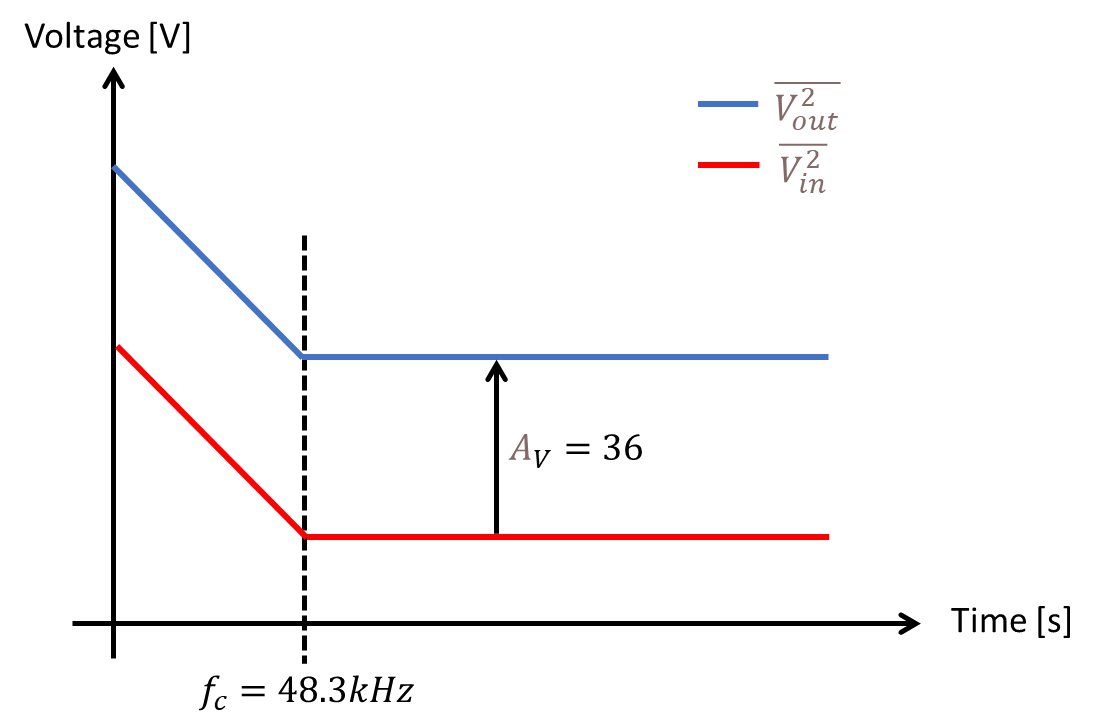
\includegraphics[width=.9\linewidth]{img/q1/sketch.png}
\caption{\label{fig:sketch-q2}Sketch}
\end{figure}

\item RMS integrated output noise voltage,

\begin{equation*}
\begin{aligned}
v_{rms, noise, out} &= \sqrt{\int_{10^{3}}^{10 \times 10^6}  \frac{K(g_{m}R_{D})^{2}}{C_{OX}WL} \cdot \frac{1}{f} \,df + 4kTR_{D}^{2}(\gamma{}g_{m} + \frac{1}{R_{D}})\Delta{}f} \\
&= \sqrt{[\frac{K(g_{m}R_{D})^{2}}{C_{OX}WL} ln(f) + 4kTR_{D}^{2}(\gamma{}g_{m} + \frac{1}{R_{D}})]_{10^{3}}^{10 \times 10^6}} \\
&= 9.30 \times 10^{-5} \frac{V}{\sqrt{Hz}}
\end{aligned}
\end{equation*}

\item RMS integrated output noise voltage,

\begin{equation*}
\begin{aligned}
v_{rms, noise, out} &= \sqrt{\int_{10^{3}}^{10 \times 10^6}  \frac{K(g_{m}R_{D})^{2}}{C_{OX}WL} \cdot \frac{1}{f} \,df + 4kTR_{D}^{2}(\gamma{}g_{m} + \frac{1}{R_{D}})\Delta{}f} \\
&= \sqrt{[\frac{K(g_{m}R_{D})^{2}}{C_{OX}WL} ln(f) + 4kTR_{D}^{2}(\gamma{}g_{m} + \frac{1}{R_{D}})]_{10^{3}}^{10 \times 10^{3}}} \\
&=  9.98 \times 10^{-6} \frac{V}{\sqrt{Hz}}
\end{aligned}
\end{equation*}

\item SNR,

\begin{equation*}
\begin{aligned}
SNR &= 20log(\frac{V_{rms,signal}}{V_{rms,noise}}) \\
&= 80 dB \\
\end{aligned}
\end{equation*}
\end{enumerate}

\section{Problem 2}
\label{sec:org6110393}
Output resistance, transconductance and gain of amplifier,
\begin{equation*}
\begin{aligned}
R_{out} &= (r_{o} + R_{s}) + g_{m}R_{s}r_{o} \\
G_{m} &= \frac{g_{m}}{(1 + \frac{R_{s}}{r_{o}}) + g_{m}R_{s}} \\
A_{V} &= \frac{g_{m}[(r_{o} + R_{s}) + g_{m}R_{s}r_{o}]}{(1 + \frac{R_{s}}{r_{o}}) + g_{m}R_{s}}\\
\end{aligned}
\end{equation*}

\begin{enumerate}[(a)]
\item Thermal noise from:

Transistor, \(M\)
\begin{equation*}
\begin{aligned}
\overline{v_{M, out}^2} &= 4kT\gamma{}g_{m}R_{out}^{2} \\
&= 4kT\gamma{}g_{m}[(r_{o} + R_{s}) + g_{m}R_{s}r_{o}]^{2} \\
\end{aligned}
\end{equation*}

Resistor, \(R_{S}\)
\begin{equation*}
\begin{aligned}
\frac{V_{S} - V_{o}}{r_{o}} = -g_{m}V_{s} \\
V_{o} = (1 + g_{m}r_{o})V_{s} \\
\\
\overline{v_{R_{s}, out}^2} &= 4kTR_{s}(1 + g_{m}r_{o})^{2} \\
\end{aligned}
\end{equation*}

Total output noise voltage,
\begin{equation*}
\begin{aligned}
\overline{v_{n, out}^2} &= 4kT\gamma{}g_{m}[(r_{o} + R_{s}) + g_{m}R_{s}r_{o}]^{2} + 4kTR_{s}(1 + g_{m}r_{o})^{2} \\
\end{aligned}
\end{equation*}

\item Ratio between thermal noise,

\begin{equation*}
\begin{aligned}
\frac{\overline{v_{M, out}^2}}{\overline{v_{R_{s}, out}^2}} &= \frac{4kT\gamma{}g_{m}[(r_{o} + R_{s}) + g_{m}R_{s}r_{o}]^{2}}{4kTR_{s}(1 + g_{m}r_{o})^{2}} \\
&= \frac{\gamma{}g_{m}[(r_{o} + R_{s}) + g_{m}R_{s}r_{o}]^{2}}{R_{s}(1 + g_{m}r_{o})^{2}} \\
&\approx \gamma{}g_{m}R_{s} \\
\end{aligned}
\end{equation*}

\item Input referred thermal noise,

\begin{equation*}
\begin{aligned}
\overline{v_{n, in}^2} &= \frac{\overline{v_{n, out}^2}}{A_{v}^{2}} \\
&= \{4kT\gamma{}g_{m}[(r_{o} + R_{s}) + g_{m}R_{s}r_{o}]^{2} + 4kTR_{s}(1 + g_{m}r_{o})^{2}\}[\frac{(1 + \frac{R_{s}}{r_{o}}) + g_{m}R_{s}}{g_{m}[(r_{o} + R_{s}) + g_{m}R_{s}r_{o}]}]^{2}\\
&= 6.4653 \times 10^{-16} \frac{V^{2}}{Hz}
\end{aligned}
\end{equation*}
\end{enumerate}

\section{Problem 3}
\label{sec:org1eaf60e}

\begin{enumerate}[(a)]
\item Since the circuit is symmetrical the differential noise due to the current mirrors, M\textsubscript{N3} and M\textsubscript{N4}
is 0.
\begin{equation*}
\begin{aligned}
\overline{v_{n, diff, out}^2} &= 0 \frac{V^{2}}{Hz} \\
\end{aligned}
\end{equation*}

\item Common mode noise at output.

Noise current spectrum density at source of \(M_{N_{4}}\),
\begin{equation*}
\begin{aligned}
\overline{i_{n, M_{N3}}^2} &= \frac{4kT\gamma{}g_{m4}^{2}}{g_{m3}} \\
\overline{i_{n, M_{N4}}^2} &= 4kT\gamma{}g_{m4} \\
\overline{i_{n}^{2}} &= \frac{4kT\gamma{}g_{m4}^{2}}{g_{m3}} + 4kT\gamma{}g_{m4} \\
&= 4kT\gamma{}g_{m4}(1 + \frac{g_{m4}}{g_{m3}}) \\
\end{aligned}
\end{equation*}

Input referred noise voltage,
\begin{equation*}
\begin{aligned}
\overline{v_{n, in}^{2}} &= \frac{\overline{i_{n}^{2}}}{4g_{m1}^{2}} \\
&= \frac{g_{m4}kT\gamma{}}{g_{m1}^{2}}(1 + \frac{g_{m4}}{g_{m3}}) \\
\end{aligned}
\end{equation*}

Output referred common-mode noise,
\begin{equation*}
\begin{aligned}
A_{CM-CM}(s) &= \frac{-g_{m1}}{g_{m2} + sC_{L}} \\
\\
\overline{v_{n, out}^{2}} &= \overline{v_{n, in}^{2}} A_{CM-CM}(s)^2 \\
&= \frac{g_{m4}kT\gamma{}}{g_{m1}^{2}}(1 + \frac{g_{m4}}{g_{m3}})[\frac{g_{m1}}{g_{m2} + sC_{L}}]^{2} \\
&= \frac{g_{m4}kT\gamma{}}{(g_{m2} + sC_{L})^{2}}(1 + \frac{g_{m4}}{g_{m3}}) \\
&= \frac{2g_{m4}kT\gamma{}}{(g_{m2} + sC_{L})^{2}} \\
\end{aligned}
\end{equation*}

Doubling \(I_{B}\) and \(W_{3}\), will not increase the current at the amplifier or \(g_{m3}\).
Therefore
\begin{equation*}
\begin{aligned}
\overline{v_{n, out}^{2}} &= \frac{g_{m4}kT\gamma{}}{(g_{m2} + sC_{L})^{2}}(1 + \frac{g_{m4}}{g_{m3}}) \\
&= \frac{2g_{m4}kT\gamma{}}{(g_{m2} + sC_{L})^{2}} \\
\end{aligned}
\end{equation*}

\item Total differential input and output noise PSD,

\begin{equation*}
\begin{aligned}
Z_{out}(s) &= \frac{1}{g_{m2} + sC_{L}} \\
A_{DM-DM} &= \frac{g_{m1}}{g_{m2} + sC_{L}} \\
\\
\overline{v_{n, MN1 \& MN2}(s)^{2}} &= (\frac{1}{g_{m2} + sC_{L}})^{2}(4kT\gamma{}g_{m1} + 4kT\gamma{}g_{m1}) \\
&= \frac{8kT\gamma{}g_{m1}}{(g_{m2} + sC_{L})^{2}} \\
\\
\overline{v_{n, MP1 \& MP2}(s)^{2}} &= (\frac{1}{g_{m2} + sC_{L}})^{2}(4kT\gamma{}g_{m2} + 4kT\gamma{}g_{m2}) \\
&= \frac{8kT\gamma{}g_{m2}}{(g_{m2} + sC_{L})^{2}} \\
\\
\overline{v_{n,out}^{2}}(s) &= \frac{8kT\gamma{}}{(g_{m2} +sC_{L})^{2}}(g_{m1} + g_{m2}) \\
\\
\overline{v_{n,in}^{2}} &= \frac{8kT\gamma{}}{g_{m1}^{2}}(g_{m1} + g_{m2}) \\
\end{aligned}
\end{equation*}

\item Integrated differential output thermal noise,

\begin{equation*}
\begin{aligned}
\overline{v_{n,out}^{2}}(s) &= \frac{8kT\gamma{}}{(g_{m2} +sC_{L})^{2}}(g_{m1} + g_{m2}) \\
&= \frac{8kT\gamma{}(g_{m1} + g_{m2})}{g_{m2}^{2}(1 +\frac{sC_{L}}{g_{m2}})^{2}} \\
&= \frac{8kT\gamma{}(g_{m1} + g_{m2})}{g_{m2}^{2}} \frac{1}{(1 +\frac{sC_{L}}{g_{m2}})^{2}} \\
\\
ENBW &= \frac{\pi}{2}\frac{g_{m2}}{2\pi{}C_{L}} \\
&= \frac{g_{m2}}{4C_{L}} \\
\\
v_{rms}^2 &= \frac{8kT\gamma{}(g_{m1} + g_{m2})}{g_{m2}^{2}} \times ENBW \\
&= \frac{2kT\gamma{}(g_{m1} + g_{m2})}{g_{m2}C_{L}} \\
\end{aligned}
\end{equation*}

\item Integrated differential output thermal noise,

\begin{equation*}
\begin{aligned}
v_{rms}^2 &= \frac{8kT\gamma{}(g_{m1} + g_{m2})}{g_{m2}^{2}} \times ENBW \\
&= \frac{2kT\gamma{}(g_{m1} + g_{m2})}{g_{m2}C_{L}} \\
&= 2.76 \times 10^{-08} \frac{V^{2}}{Hz}
\end{aligned}
\end{equation*}
\end{enumerate}


\section{Problem 4}
\label{sec:org294a3a5}
Gain, cutoff frequency, BW, and ENBW of amplifier

\begin{equation*}
\begin{aligned}
A_{DM-DM} &= \frac{g_{m1}}{g_{m2} + sC_{L}} \\
f_{c} &= \frac{g_{m2}}{2\pi{}C_{L}} \\
ENBW &= \frac{g_{m2}}{4C_{L}} \\
\end{aligned}
\end{equation*}


Steps taken for determining the dimensions of transistors.
\begin{enumerate}
\item Select values so that the gain, \(|A_{v} \geq 5|\). The tail current is increased when the dimensions exceeds
the allowed limit in the model, by doing so the transconductance is increased without increasing the dimensions.
\item The capacitance of the output capacitance is selected to give a cutoff of \(f_{c} \geq 2MHz\).
\item The 1/f noise corner is decreased below, \(f_{c} \leq 100kHz\), by changing the
dimensions of the transistors but keeping the ratio of W/L constant.
\item The total integrated noise is from 1Hz to 100MHz is \(52.675 \mu{}V\).
\end{enumerate}

Final dimensions of transistors and bias current
\begin{center}
\begin{tabular}{ll}
\hline
\(I_{B}\) & \(0.05mA\)\\
\hline
\(W_{N1}\) & \(80um\)\\
\(L_{N1}\) & \(2um\)\\
\(W_{N2}\) & \(80um\)\\
\(L_{N2}\) & \(2um\)\\
\hline
\(W_{N3}\) & \(20um\)\\
\(L_{N3}\) & \(2um\)\\
\(W_{N4}\) & \(20um\)\\
\(L_{N4}\) & \(2um\)\\
\hline
\(W_{P1}\) & \(20um\)\\
\(L_{P1}\) & \(2um\)\\
\(W_{P2}\) & \(20um\)\\
\(L_{P2}\) & \(2um\)\\
\hline
\end{tabular}
\end{center}

Testbench of amplifier
\begin{figure}[H]
\centering
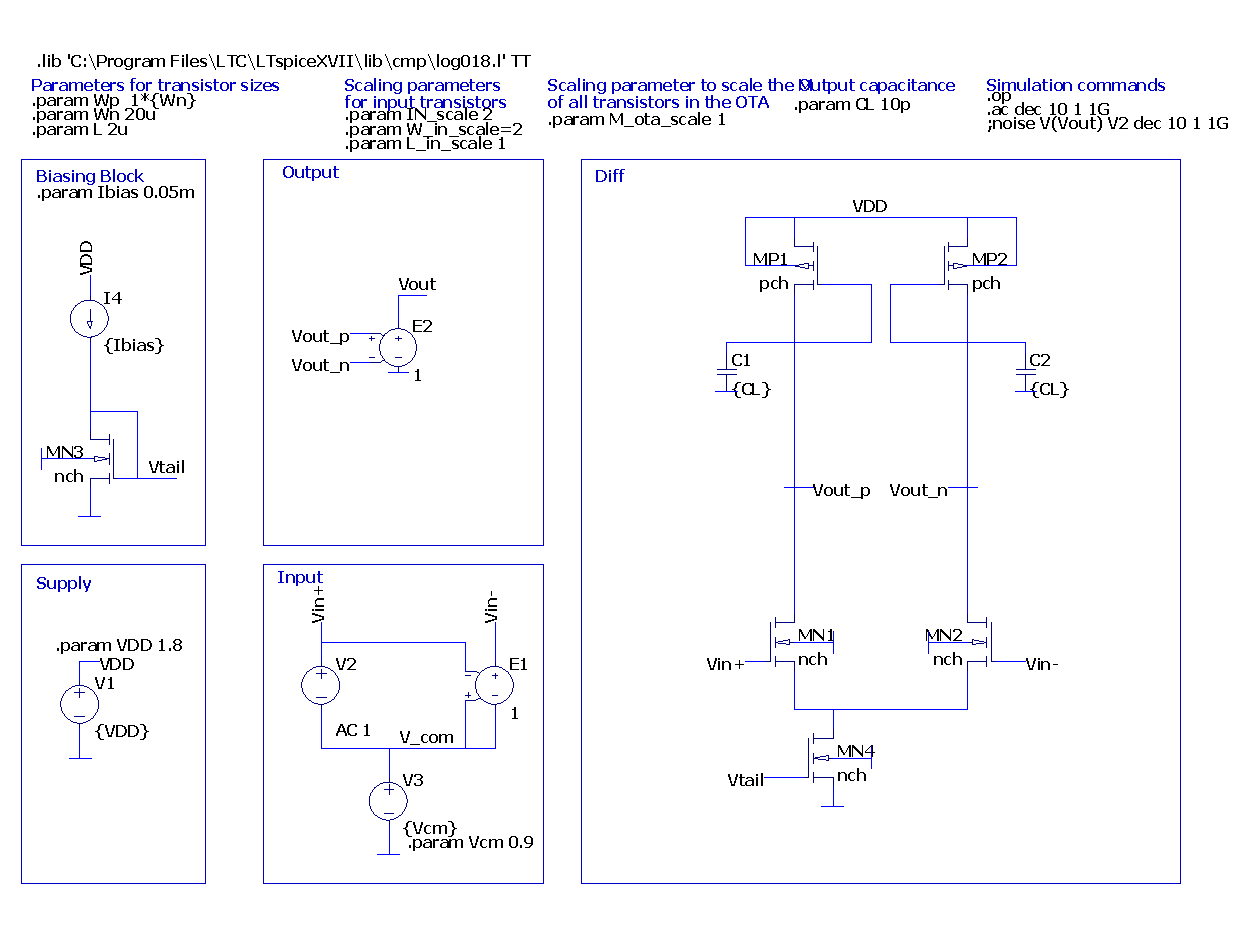
\includegraphics[height=300px]{img/q4/testbench.pdf}
\caption{\label{fig:testbench-q4}Testbench}
\end{figure}

Gain of amplifier
\begin{figure}[H]
\centering
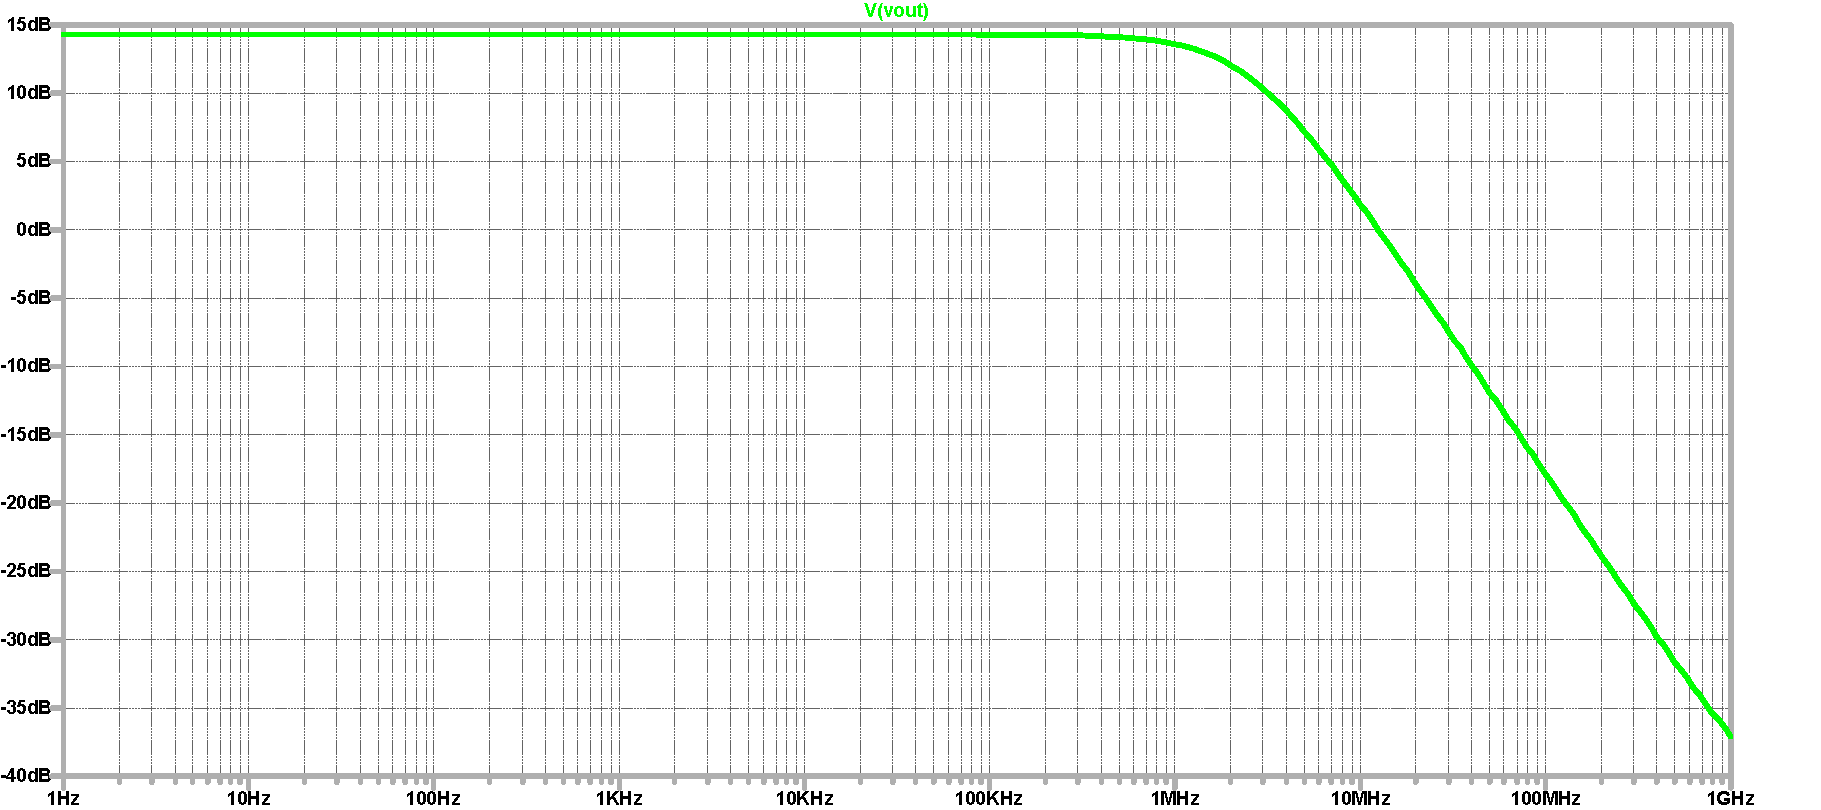
\includegraphics[width=.9\linewidth]{img/q4/gain.pdf}
\caption{\label{fig:gain-q4}Gain}
\end{figure}

Noise analysis
\begin{figure}[H]
\centering
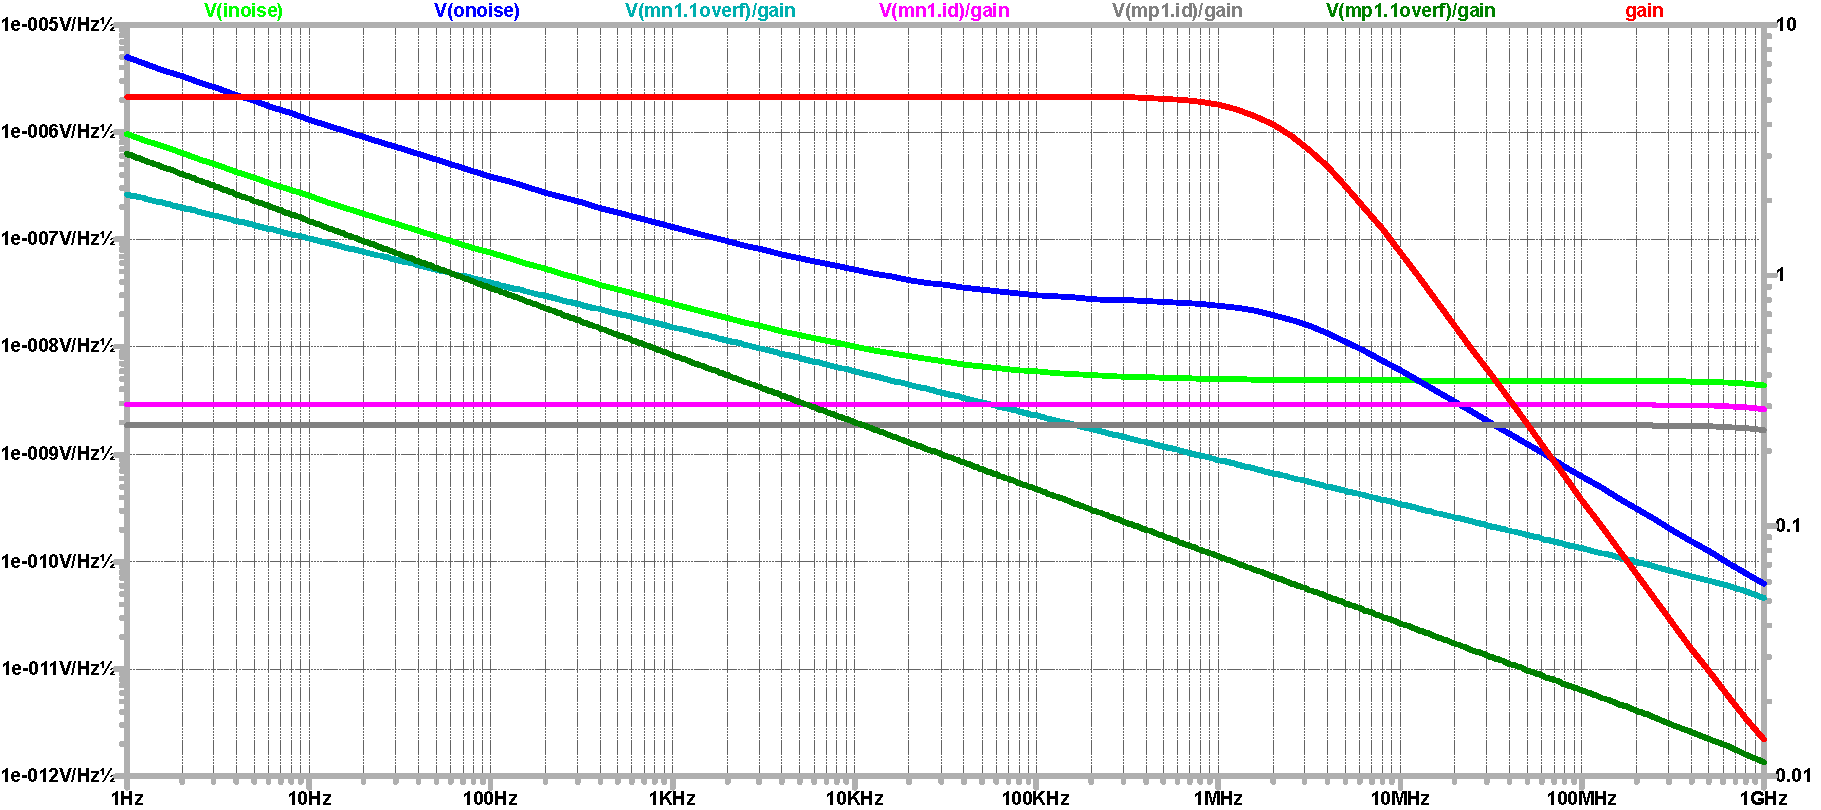
\includegraphics[width=.9\linewidth]{img/q4/noise.pdf}
\caption{\label{fig:noise-q4}Noise analysis}
\end{figure}

Transient analysis
\begin{figure}[H]
\centering
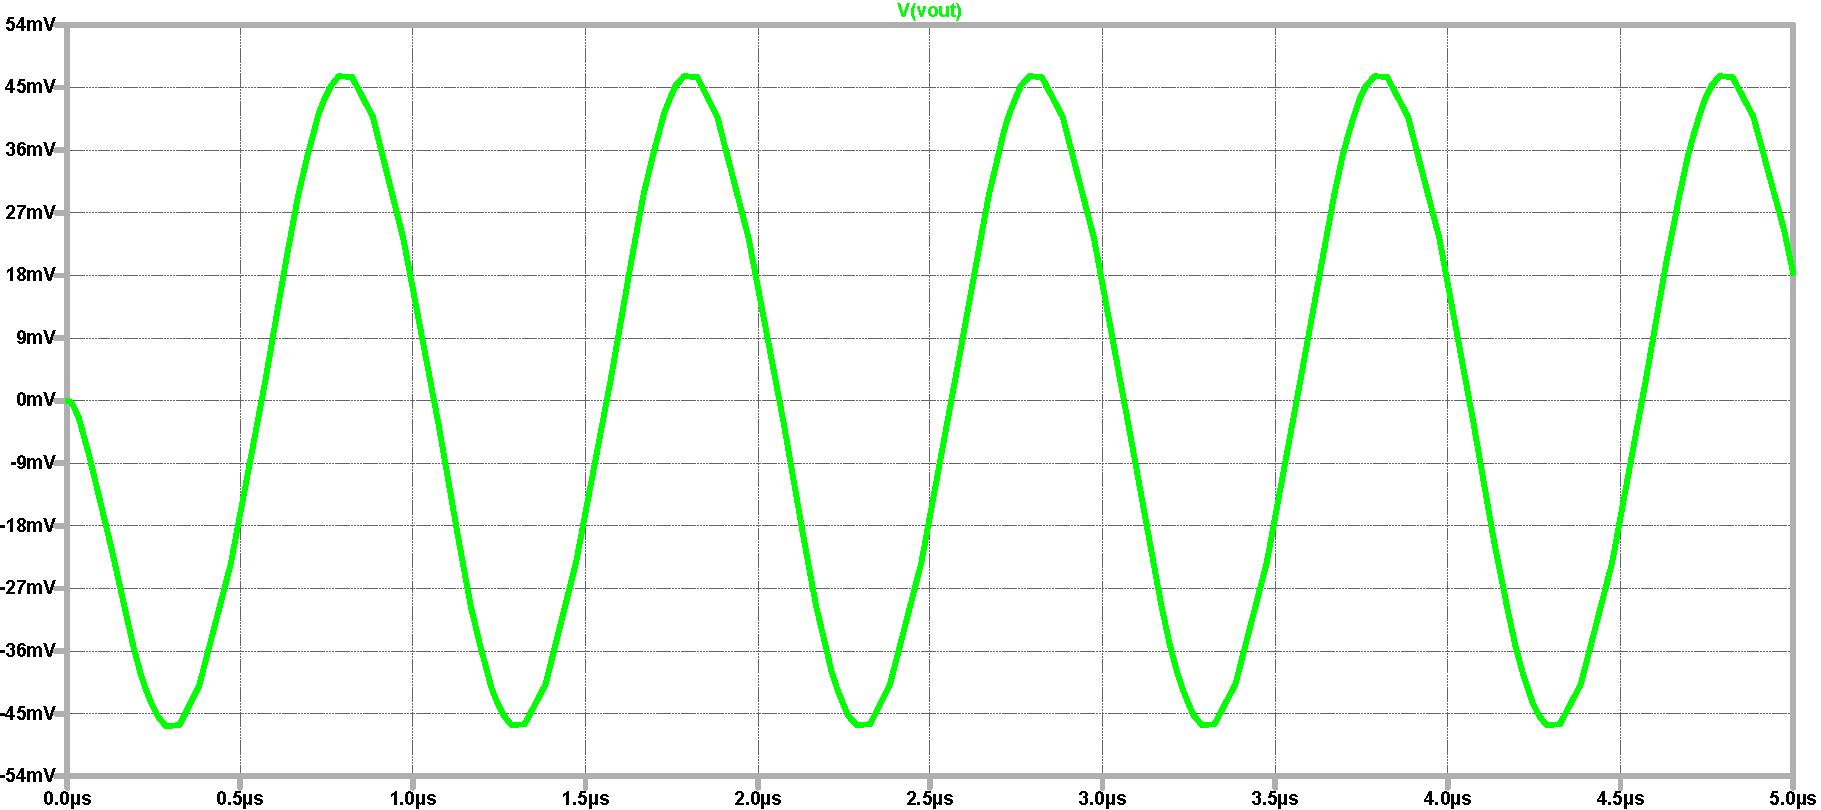
\includegraphics[width=.9\linewidth]{img/q4/trans.pdf}
\caption{\label{fig:transient-q4}Transient analysis}
\end{figure}

Final results of amplifier,
\begin{center}
\begin{tabular}{ll}
\hline
Small-signal Gain, \(A_{V}\) & 5.17\\
3dB bandwidth, \(f_{-3dB}\) & 2.4 MHz\\
Integrated output noise from 1Hz to 100MHz & \(52.675 \mu{}V\)\\
1/f noise corner & 50.7 KHz\\
\hline
\end{tabular}
\end{center}
\end{document}
